\chapter{Plataforma Eventos IFF} \label{cap:eventosiff}

Eventos IFF é uma plataforma \textit{web} voltada para o processo de criação, divulgação e gestão de eventos acadêmicos. A plataforma tem uma arquitetura planejada para funcionar através de uma comunicação via serviços, havendo assim comunicações externas para realização de algumas funcionalidades.

A etapa inicial do ciclo de vida do evento na plataforma é iniciado com a solicitação de criação do mesmo, que é avaliada, podendo assim ser aprovada ou reprovada sua criação através do Sistema de Gestão Integrado, chamado de Sistema Unificado de Administração Pública (SUAP).

Posteriormente a criação e aprovação do evento, o mesmo pode ser gerenciado através do \textit{website}. Este gerenciamento conta com funcionalidades, tais como: ativação do evento, cadastro de atividades e administração do portal do evento.

Como resultado da disponibilidade do evento na plataforma, o mesmo pode receber inscrições em suas atividades. O Eventos IFF também possibilita a submissão de trabalhos científicos dos seus participantes, permitindo serem avaliados pela a administração do evento.

Decorrente do início do evento, o Eventos IFF oferece suporte para funcionalidades com o intuito de realizar o credenciamento dos participantes nas atividades realizadas pelo o mesmo. Acrescentando-se que, a plataforma, por meio de comunicação com os serviços do E-certificados, permite a geração e envio dos certificados de participação nas atividades e no evento.

Na Figura \ref{fig:eventosiff} é apresentado um fluxograma ilustrando as etapas no processo de gerenciamento de eventos, como descrito nesse capítulo.

\begin{figure}[H]
    \centering
    \caption{Fluxograma das etapas de gerenciamento de eventos no Eventos IFF}
    % 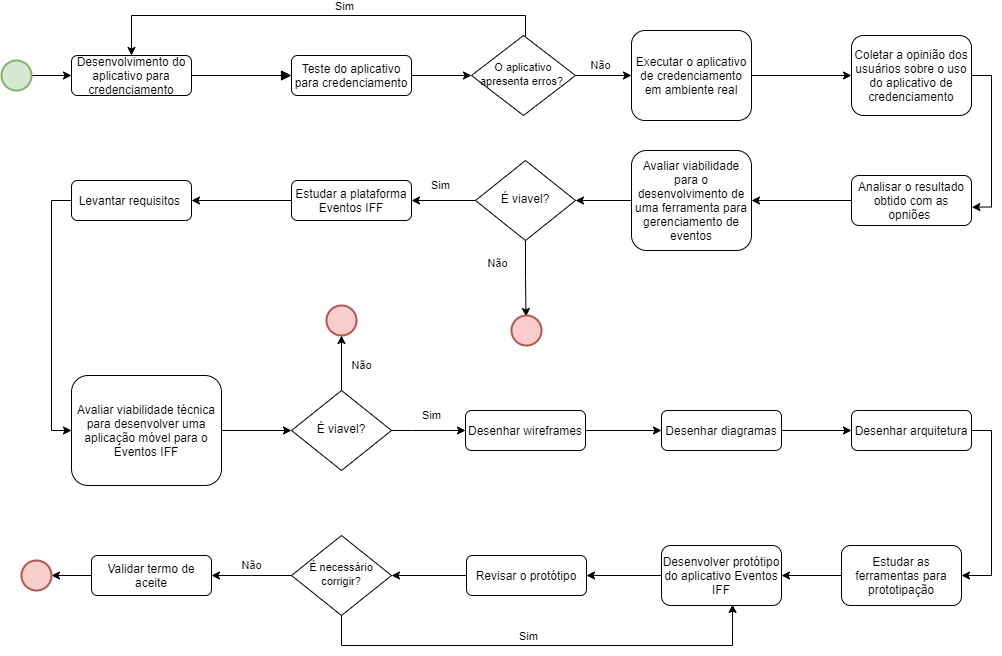
\includegraphics[scale=0.45]{figuras/metodologia.jpg}
    \fbox{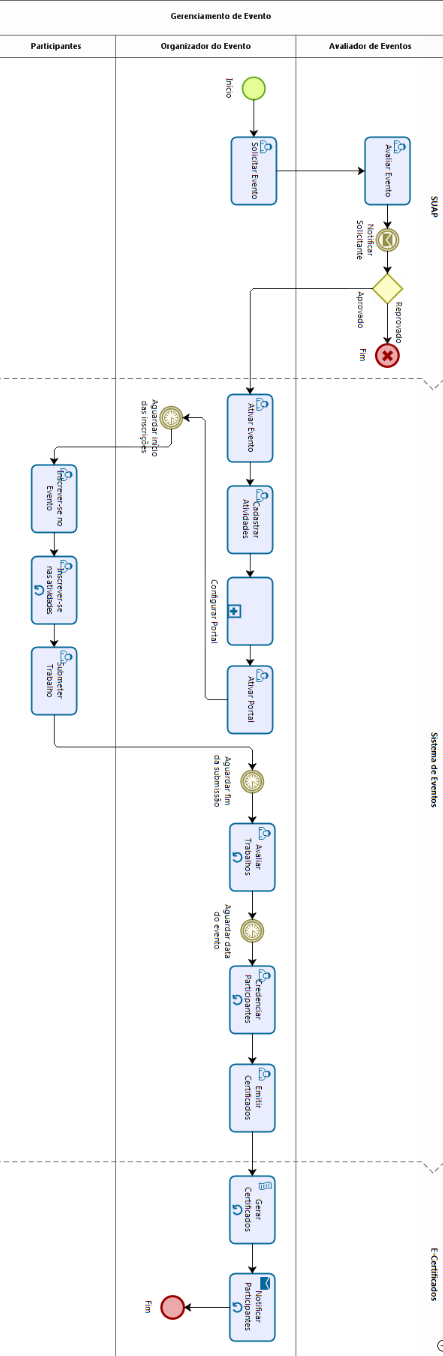
\includegraphics[scale=0.5]{figuras/eventos-iff.png}}
    \label{fig:eventosiff}
    \legend{Fonte: Instituto Federal Fluminense}
\end{figure}

No fluxograma da Figura \ref{fig:eventosiff}, é possível visualizar a atuação das integrações externas, sendo elas o SUAP e o E-certificados, assim como a divisão dos usuários participantes e organizadores.

Concluindo, como mencionado anteriormente, o Eventos IFF atua através de um \textit{website}, permitindo a realização de todas as funcionalidades descritas neste capítulo. Entretanto, não dispõe de uma aplicação para dispositivos móveis. 



